\documentclass{article}

% Language setting
% Replace `english' with e.g. `spanish' to change the document language
\usepackage[english]{babel}

% Set page size and margins
% Replace `letterpaper' with `a4paper' for UK/EU standard size
\usepackage[letterpaper,top=2cm,bottom=2cm,left=3cm,right=3cm,marginparwidth=1.75cm]{geometry}

% Useful packages
\usepackage{amsmath}
\usepackage{graphicx}
\usepackage[colorlinks=true, allcolors=blue]{hyperref}

\title{Predicting Tyre Compound Quality using Logistic Regression}
\author{Md Zakir Hossain}

\begin{document}
\maketitle

\begin{abstract}
The quality of a tyre compound is crucial for both the safety of drivers and the tyre industry. However, the traditional method of evaluating tyre compound quality is time-consuming and requires expert judgment. With the rise of machine learning, we can automate these tasks and replace human experts with computational models.
My project focuses on predicting the quality of tyre compounds using logistic regression, KNN, SVM, and ANN. However, not all features are relevant for better prediction, so we will focus on identifying the important features that contribute to accurate prediction.
To evaluate the performance of our models, i will use one dataset containing information about tyre compound quality. To determine feature importance, i will use correlation coefficients such as Pearson's coefficient, along with performance metrics such as accuracy, recall, precision, and f1 score. We will also apply a grid search algorithm to improve the model's accuracy.
After evaluating the machine learning algorithms, i found that the ANN algorithm outperformed the SVM and KNN algorithms in predicting tyre compound quality for dataset.
.
\end{abstract}

\section{Itroduction}

The quality of the tyre compound is a very important part for the consumers as well as the manufacturing industries. Industries are increasing their sales using product quality certification. Nowadays, all over the world tyre is a regularly used items and the industries are using the certification of product quality to increases their value in the market. Previously, testing of product quality will be done at the end of the production, this is time taking process and it requires a lot of resources such as the need for various human experts for the assessment of product quality which makes this process very expensive. Every human has their own opinion about the test, so identifying the quality of the tyre compound  based on humans experts it is a challenging task. There are several features to predict the tyre compound quality but the entire features will not be relevant for better prediction. The project aims to what tyre compound features are important to get the promising result by implementing the different machine learning algorithms such as logistic regression, support vector machines (SVMs), k-nearest neighbors (KNN), and artificial neural networks (ANNs) using a logistic activation function on the final layer.
using the tyre compound quality dataset. 


\begin{figure}[ht!]
  \centering
  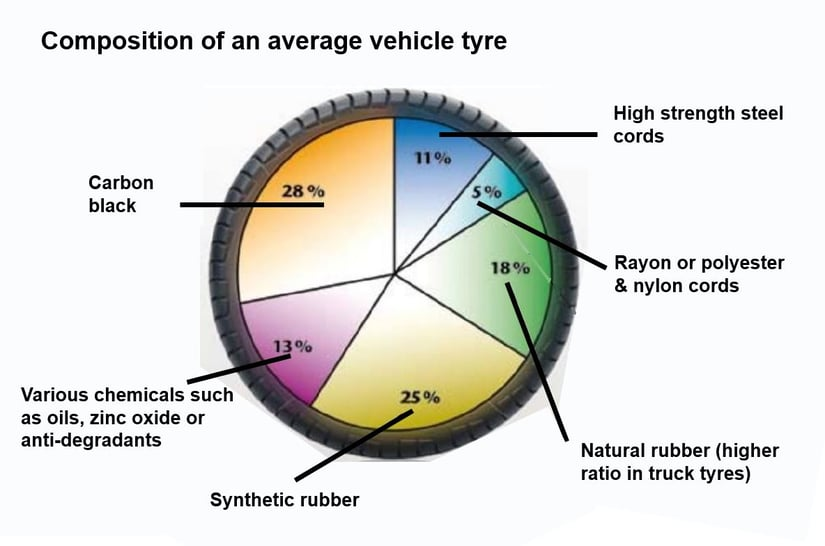
\includegraphics[width=0.6\textwidth]{tyre.jpg}
  \caption{Composition of tyre}
\end{figure}





\begin{table}
\centering
\begin{tabular}{l|r}
Item & Quantity \\\hline
Carbon & 28\% \\
Chemicals & 13\% \\
NR+SBR & 43\%
\end{tabular}
\caption{\label{tab:widgets}An example table.}
\end{table}

I collect the tyre quality dataset from my previous company, and I collect some data from different websites. The dataset contains a small collection of datasets. The tyre compound dataset contains 65 instances and the file contain 13 input features and 1 output feature. Input features are based on the tests and output variable based on sensory data is scaled in 8 quality classes from 2 to 8 (2-very bad to 8-very good). 

\section{Background}

 A wide range of machine learning algorithms is available for the learning process. This section describes the classification algorithms used in tyre compound quality prediction and related work.

 \subsection{Classification algorithm }

 \subsection{Logistic Regression}

Logistic regression uses a logistic function called a sigmoid function to map predictions and their probabilities. The sigmoid function refers to an S-shaped curve that converts any real value to a range between 0 and 1.

Moreover, if the output of the sigmoid function (estimated probability) is greater than a predefined threshold on the graph, the model predicts that the instance belongs to that class. If the estimated probability is less than the predefined threshold, the model predicts that the instance does not belong to the class.

For example, if the output of the sigmoid function is above 0.5, the output is considered as 1. On the other hand, if the output is less than 0.5, the output is classified as 0. Also, if the graph goes further to the negative end, the predicted value of y will be 0 and vice versa. In other words, if the output of the sigmoid function is 0.65, it implies that there are 65% chances of the event occurring; a coin toss, for example.

The sigmoid function is referred to as an activation function for logistic regression and is defined as:

$f(x) = \frac{1}{1+ e^{-x}}$

where,

e = base of natural logarithms

value = numerical value one wishes to transform.

The following equation represents logistic regression:

$y= \frac{e^{b_0+b_1x}}{1+ e^{b_0+b_1x} }$

Logistic Regression – Sigmoid Function

here,

x = input value

y = predicted output

b0 = bias or intercept term

b1 = coefficient for input (x)


\begin{figure}[h!]
  \centering
  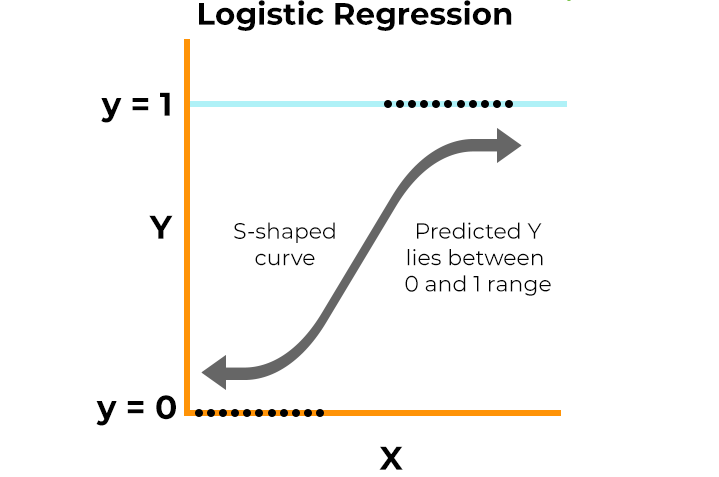
\includegraphics[width=0.6\textwidth]{logistic.png}
  \caption{Logistic curve.}
\end{figure}

 

\subsubsection{Support Vector Machine}

 The support vector machine (SVM) is the most popular and most widely used machine learning algorithm. It is a supervised learning model that can perform classification and regression tasks. However, it is primarily used for classification problems in machine learning (Gandhi, 2018). The SVM algorithm aims to create the best line or decision boundary that can separate n-dimensional space into classes. So, we can put the new data points easily in the correct groups. This best decision boundary is called a hyperplane.

\begin{figure}[h!]
  \centering
  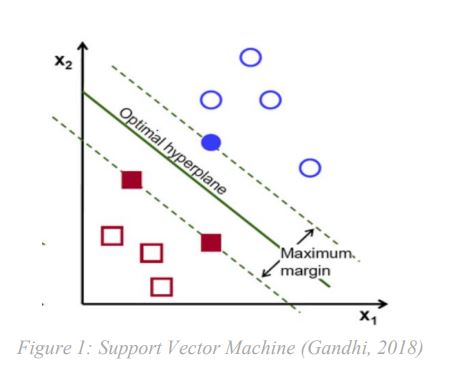
\includegraphics[width=0.6\textwidth]{svm.jpg}
  \caption{support vector machine (SVM)}
\end{figure}

Simply use the section and subsection commands, as in this example document! With Overleaf, all the formatting and numbering is handled automatically according to the template you've chosen. If you're using Rich Text mode, you can also create new section and subsections via the buttons in the editor toolbar.


The SVM model is used for both non-linear and linear data. It uses a nonlinear mapping to convert the main preparing information into a higher measurement. The model searches for the linear optimum splitting hyperplane in this new measurement. A hyperplane can split the data into two classes with an appropriate nonlinear mapping to suitably high measurements and for the finding, this hyperplane SVM uses the support vectors and edges (J. Han et al., 2012). The SVM model is a representation of the models as a point in space, the different classes are isolated by the gap to mapped with the aim that instances are wide as would be careful. The model can perform out a nonlinear form of classification (Kumar et al., 2020)

\subsection{Naive Bayesian}


The naive Bayesian is the simple supervised machine learning
classification algorithm based on the Bayes theorem. The algorithm
assumes that the feature conditions are independent of the given class
(Rish, 2001). The naive Bayes algorithm helps to build fast machine
learning models that can make a fast prediction. The algorithm finds
whether a particular portion has a spot by a particular class it utilizes
the probability of likelihood (Kumar et al., 2020).



\subsection{ANN}
The artificial neural network is a collection of neurons that can process
information. It has been successfully applied to the classification task
in several industries, including the commercial, industrial, and
scientific filed (Zhang, 2000). The algorithm model is a connection
between the neurons that are interconnected with the input layer, a
hidden layer, and an output layer (Hewahi, 2017).
5
The neural network is constant because while an element of the neural
network is failing, it can continue its parallel nature without any
difficulties (Mhatre et al., 2015).

\begin{figure}[h!]
  \centering
  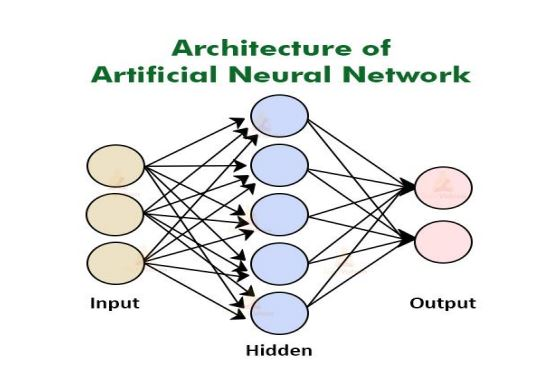
\includegraphics[width=0.6\textwidth]{ANN.jpg}
  \caption{Artificial neural network}
\end{figure}

The implementation of the artificial neural network consists of three
layers: input, hidden, and, output as shown in Figure 2. The function
at the input layer is mapped the input attribute which passes input to
the hidden layer. The hidden layer is a middle layer where all input
with the weights is received to each node in the hidden layer. The
output layer is mapped to the predicted elements (says, 2020).
The connection among the neurons is called weights, it has numerical
values and this weight among the neurons are determining the learning
ability of the neural network. The activation function is used to
standardize the output from the neurons and these activation functions
are evaluate the output of the neural network in the mathematical
equations. Each neuron has an activation function. The neural network
is hard to understand without mathematical reasoning. Activation
functions are also called the transmission function and also helps to
standardize the output range between -1 to 1 or 0 to 1.


\section{Problem}

\subsection{Problem Definition}

Based previous history, the significance of each
feature for the tyre compound quality prediction is not yet quantified. And in
terms of performance, the current accuracy is about 67.25%. Thus, in
this project, i considered two aspects of the problems mentioned
above. The first one is the study of the importance of the features for
the prediction of tyre compound quality. The secondly, performance of the
prediction model can be improved using a neural network with other
ordinary classifiers used by the articles cited above.


\subsection{Research Aim}

The following research question and hypothesis are formulated.

1. What wine features are important to get a promising result?

The researchers have used a neural network for the regression task but
for the classification task neural network was never used.
Hypothetically, the current prediction model that has been obtained by
researchers will be improved by using the neural network.


To address the research question the following objectives are
formulated :


* To balance the dataset.

* To analyze the impact of the features.


* To optimize the classification models through hyperparameter
tuning.


* To model and evaluate the approaches.

\section{Method and Approach
}

\subsection{Data Description}

Data Description
The tyre compound dataset have been used in this paper
which is obtained from my previous working company and some different websites it
contains a small collection of dataset. The dataset contains one excel file,
related to Gazi auto tyremanufacturing industries daliy tyre compound production report. The tyre compound dataset contains 65
instances. dataset have 13 input variables (based on chemical tests):
NR,	SBR	,Carbon Black,	ZnO,	Fatty Acid,	Wax	,Antizonant	,Oil,	Trackifier	,Sulfenamide	Sulfur,	Mixing Temperature,	Mixing Time,	Mixing Speed,	Total Weight , Quality Score and 1 output variable (based on testing data): quality. Sensory data is
scaled in 8 quality classes from 2 to 8 (0-very bad to 8-very good).
Below Table 1 description of the attributes.

taaaaaaaaaaaaaaaaaaaabbbbbbbbbbbbbbblllllllllllllllllleeeeeeeeeeeeeeeeeee


\subsection{Evaluation}


The performance measurement is calculated and evaluate the
techniques to detect the effectiveness and efficiency of the model.
There are four ways to check the predictions are correct or incorrect:


* True Positive: Number of samples that are predicted to be
positive which are truly positive.


* False Positive: Number of samples that are predicted to be
positive which are truly negative.


* False Negative: Number of samples that are predicted to be
negative which are truly positive.


* True Negative: Number of samples that are predicted to be
negative which are truly negative.



Below listed techniques, we use for the evaluation of the model.


1. Accuracy – Accuracy is defined as the ratio of correctly
predicted observation to the total observation. The accuracy
can be calculated easily by dividing the number of correct
predictions by the total number of predictions.

$accurecy=\frac{True Positive + True Negative}{True Positive + False Positive + False Negative + True Negative}$

2. Precision – Precision is defined as the ratio of correctly
predicted positive observations to the total predicted positive
observations.

$ Precision=\frac{True Positive }{True Positive + False Positive}$


3. Recall – Recall is defined as the ratio of correctly predicted
positive observations to all observations in the actual class.
The recall is also known as the True Positive rate calculated
as,

$  Recall=\frac{True Positive }{True Positive + False Positive}$


4. F1 Score – F1 score is the weighted average of precision and
recall. The f1 score is used to measure the test accuracy of the
model. F1 score is calculated by multiplying the recall and
precision is divided by the recall and precision, and the result
is calculated by multiplying two.

$ F1 score= 2 . \frac{Recall . Precision}{Recall + Precision}$

Accuracy is the most widely used evaluation metric for most
traditional applications. But the accuracy rate is not suitable for
evaluating imbalanced data sets, because many experts have observed
that for extremely skewed class distributions, the recall rate for
minority classes is typically 0, which means that no classification rules
are generated for the minority class. Using the terminology in
information retrieval, the precision and recall of the minority
categories are much lower than the majority class. Accuracy gives
more weight to the majority class than to the minority class, this makes
it challenging for the classifier to implement well in the minority class.

\section{Experimental design}



\subsection{Unbalanced Data}

Visualize the quality class label in the compound number and compound quality
as follows:

\begin{figure}[h!]
  \centering
  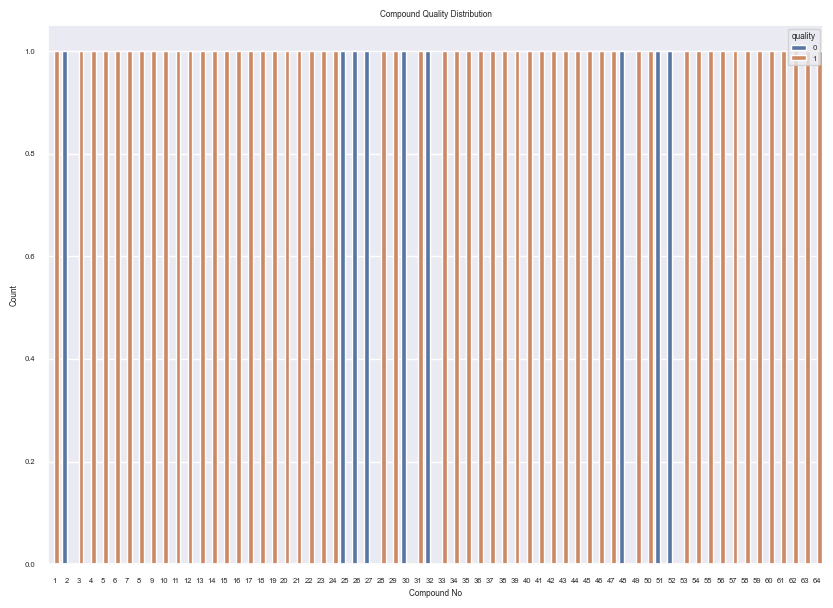
\includegraphics[width=0.8\textwidth]{unbalanced data.png}
  \caption{Unbaanced data}
\end{figure}




The code provided reads in a dataset of tyre compound data from an Excel file using Pandas. The dataset includes 16 variables, including the composition of different compounds, mixing time and speed, and quality.

The code then creates a series of bar plots using the Seaborn library to visualize the relationship between the different variables and quality. The plots show the average value of each variable for compounds with good and bad quality. These plots can help identify which variables may be most strongly related to quality


\begin{figure}[h!]
  \centering
  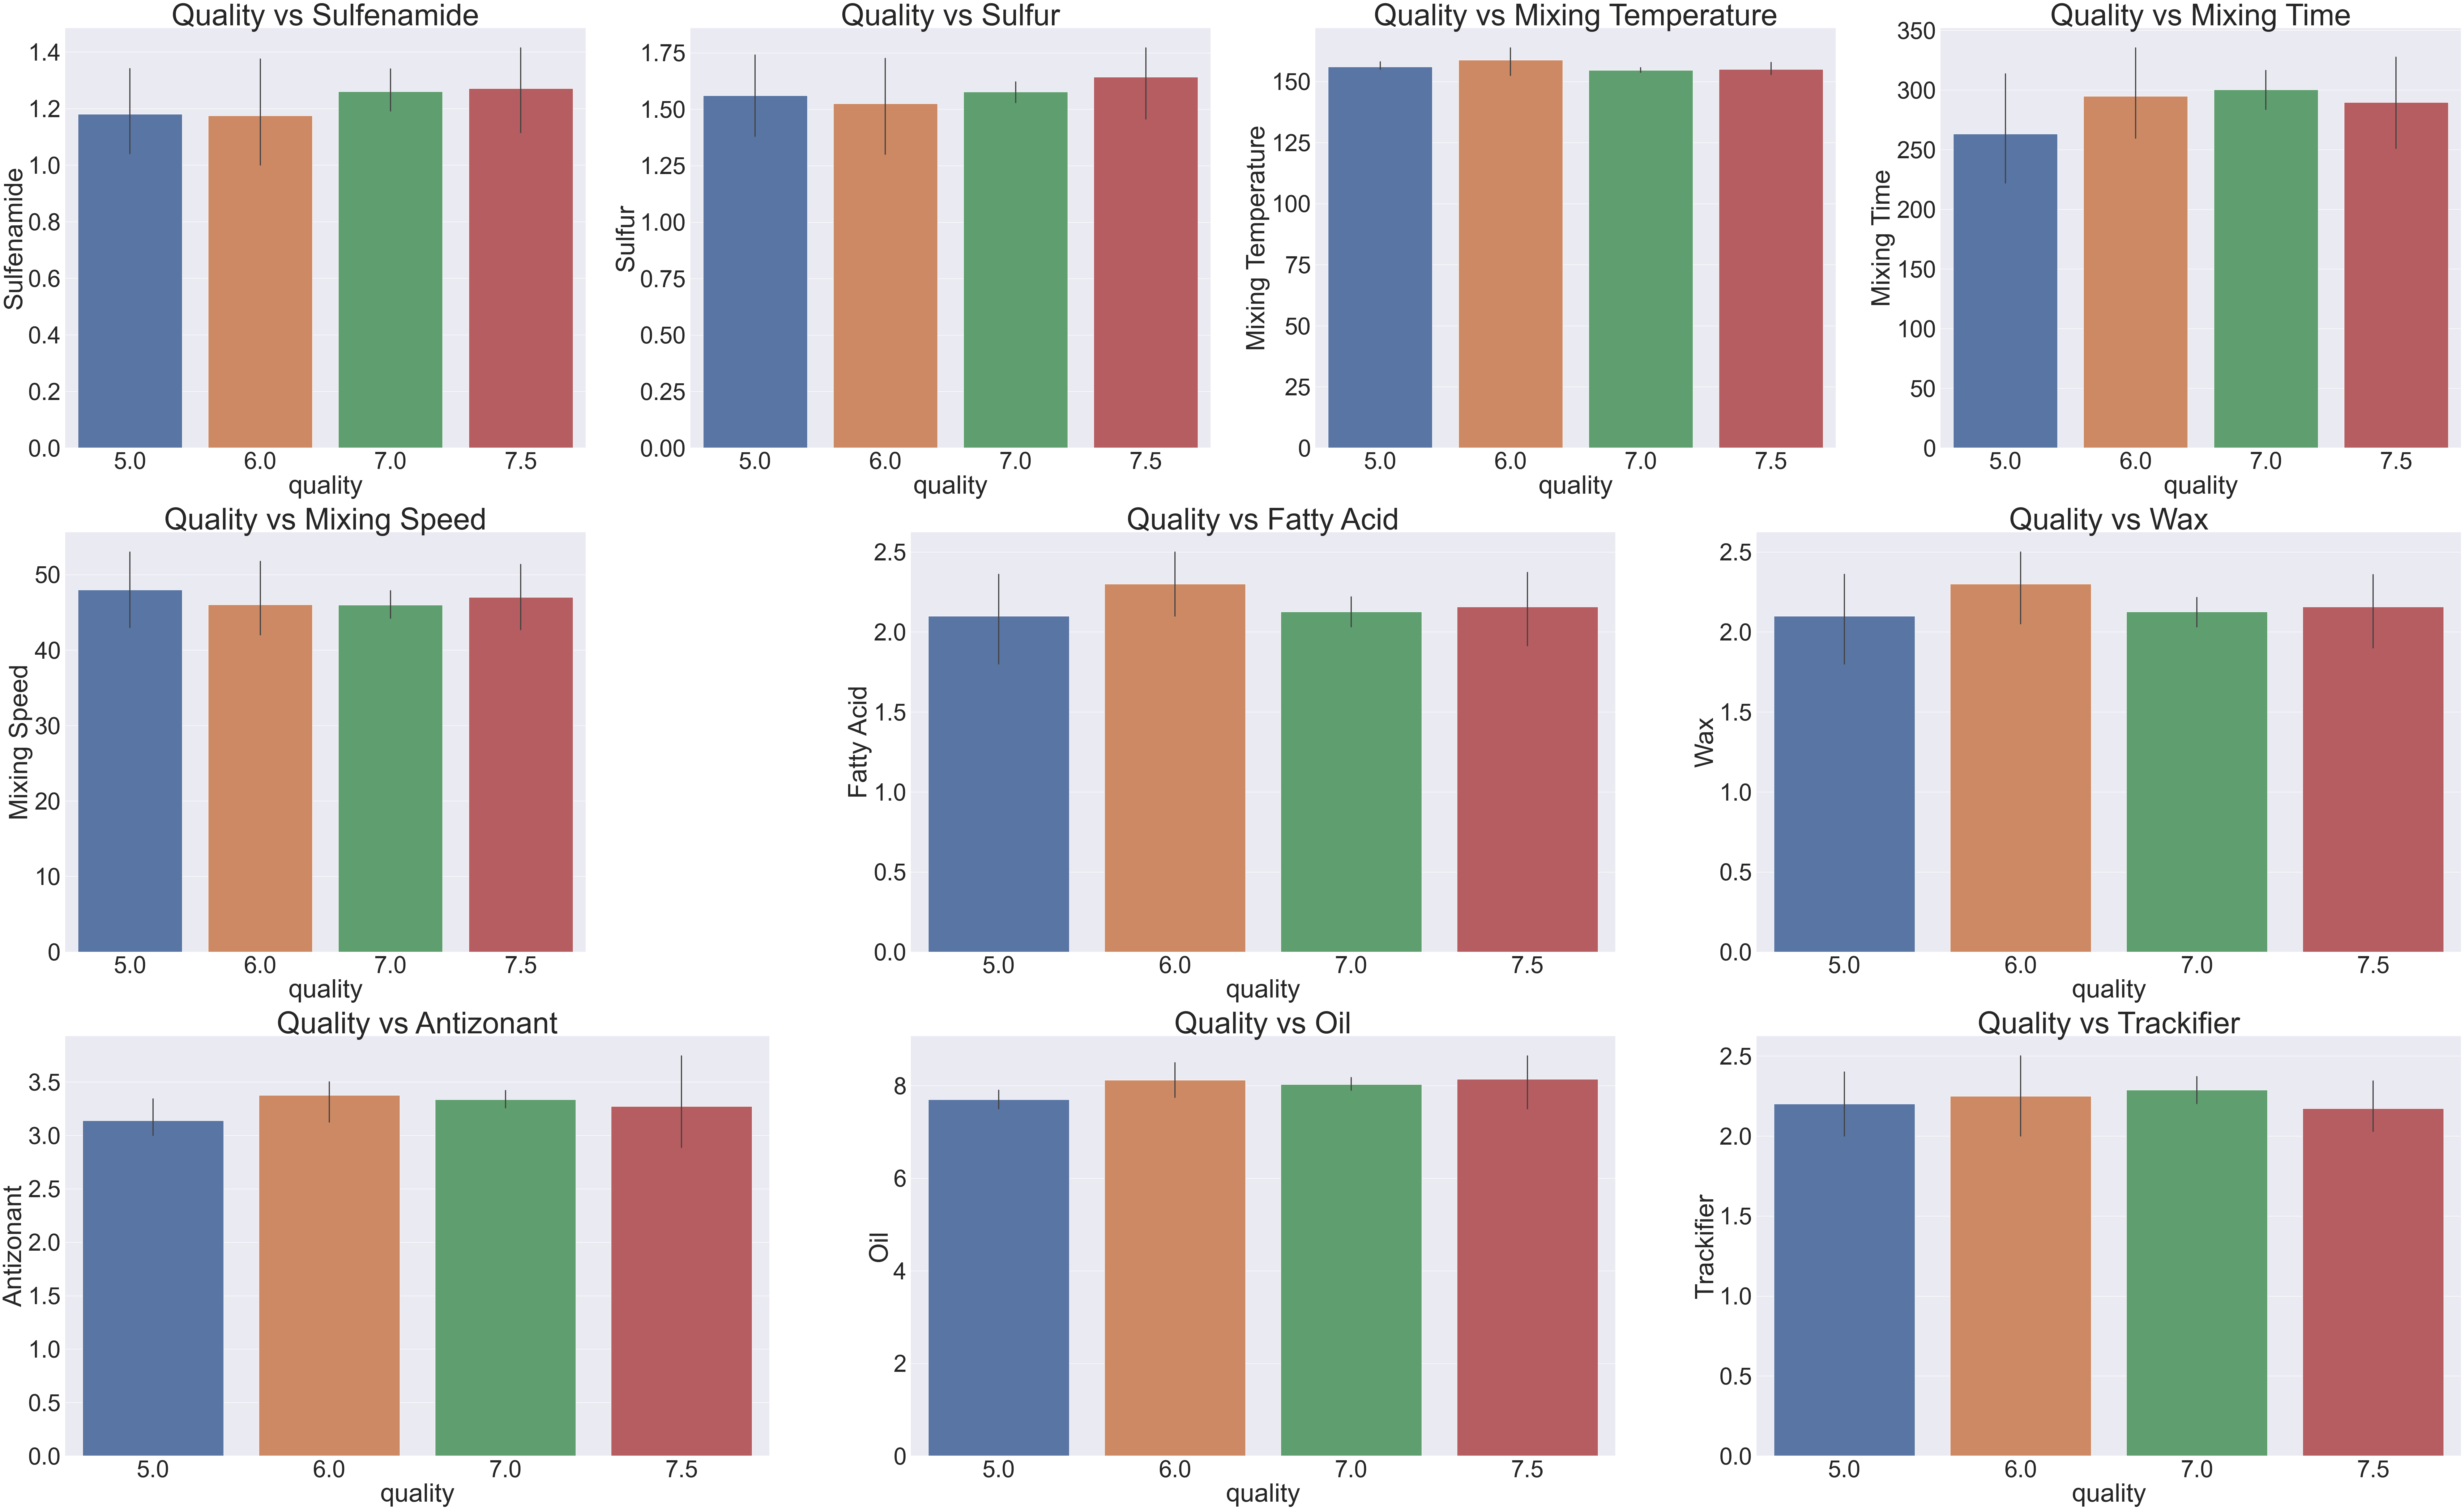
\includegraphics[width=0.8\textwidth]{1.png}
  \caption{series of bar plots using the Seaborn}
\end{figure}




\begin{figure}[h!]
  \centering
  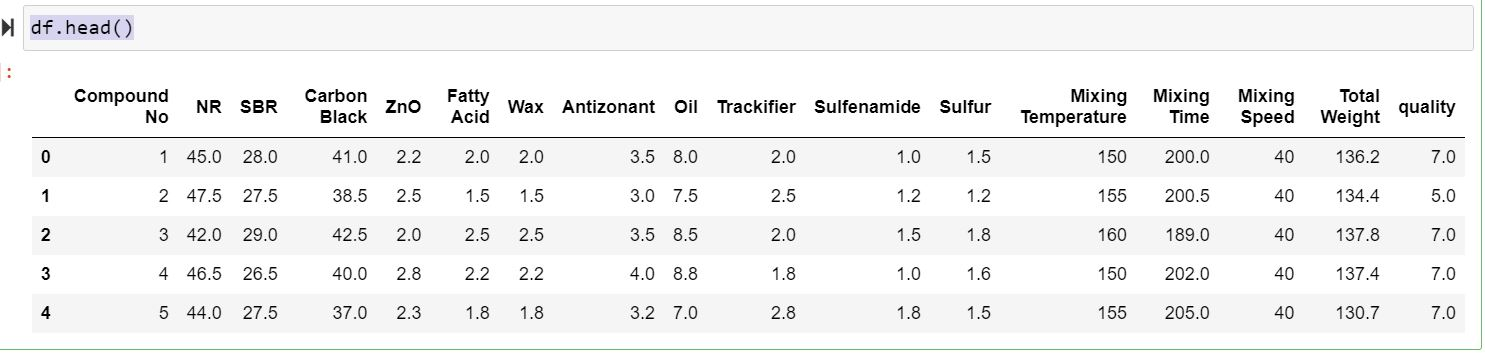
\includegraphics[width=0.8\textwidth]{df.head.jpg}
  \caption{df.head}
\end{figure}



\pagebreak
The code df.head() simply displays the first five rows of the pandas DataFrame df. It is often used as a quick way to check that the data has been imported correctly and to get a sense of what the data looks like.


I import several libraries and modules necessary for data analysis and machine learning tasks. Here is a brief explanation of each import items.

1. import pandas as pd: This imports the pandas library, which is used for data manipulation and analysis.

2. import seaborn as sns: This imports the seaborn library, which is used for data visualization and statistical graphics.

3. import matplotlib.pyplot as plt: This imports the matplotlib.pyplot module, which is used for creating visualizations such as plots and charts.

4. from sklearn.ensemble import RandomForestClassifier: This imports the RandomForestClassifier class from the sklearn.ensemble module, which is used for building random forest models.


5. from sklearn.linear model import LogisticRegression: This imports the LogisticRegression class from the sklearn.linear model module, which is used for building logistic regression models.

6. from sklearn.metrics import confusion matrix, classification report, accuracy score: This imports three functions from the sklearn.metrics module that are used for evaluating the performance of machine learning models: confusion matrix calculates the confusion matrix for a set of predictions, classification report generates a report of several classification metrics, and accuracy score calculates the accuracy of a set of predictions.


7. from sklearn.preprocessing import StandardScaler, LabelEncoder: This imports two classes from the sklearn.preprocessing module, which are used for data preprocessing tasks. StandardScaler is used for standardizing the scale of numerical features, and LabelEncoder is used for encoding categorical features into numerical values.


8. from sklearn.model selection import traintestsplit, cross val score: This imports two functions from the sklearn.model selection module. train test split is used for splitting the dataset into training and testing subsets, and cross val score is used for cross-validation, which evaluates the performance of a model on multiple subsets of the data.
Finally, import warnings and warnings.filterwarnings('ignore') are used to suppress warnings that might be generated during the execution of the code.



Then i make concise summery of a data frame . it provides information  on the number of non-null values, data types, and memory usage for each column. This method is useful in understanding the structure of the data frame, identifying missing values or inconsistent data types, and optimizing memory usage


after that, In my code, the quality column of the DataFrame df is first converted into categorical data by using pd.cut() method to bin the data into two categories: bad and good. The bins are defined as (2, 6.5, 8), meaning that any value of quality less than or equal to 6.5 will be categorized as bad, and any value greater than 6.5 will be categorized as good. The resulting categorical data is then converted into numerical labels using LabelEncoder() method, which assigns the value 0 to bad and 1 to good. The count of each label is then plotted using sns.countplot() method to visualize the distribution of quality in the dataset.


\begin{figure}[h!]
  \centering
  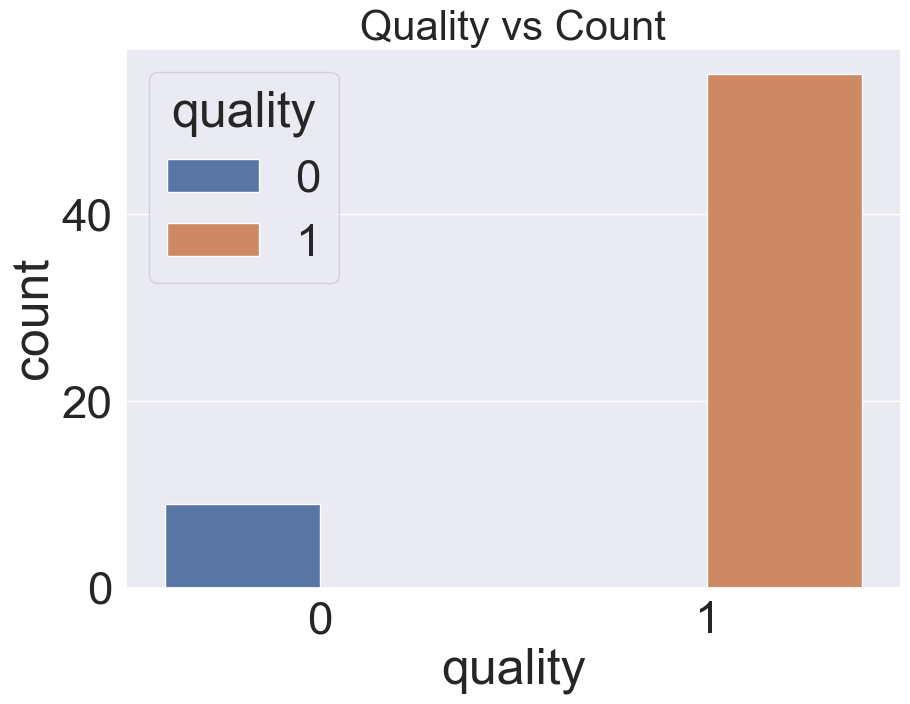
\includegraphics[width=0.8\textwidth]{good and bad.png}
  \caption{distribution of quality}
\end{figure}



\subsection{Random Forest }
 I use Random Forest Classifier model to the training data, making predictions on the test set, and evaluating the performance of the model using accuracy score and confusion matrix. The heatmap of the confusion matrix provides an easy way to visualize the performance of the model in terms of true positives, false positives, true negatives, and false negatives.




 
\begin{figure}[h!]
  \centering
  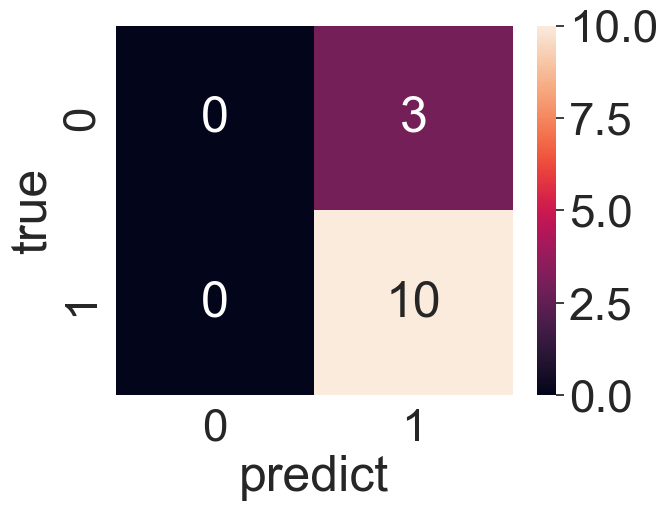
\includegraphics[width=0.8\textwidth]{heatmap.png}
  \caption{Heatmap}
\end{figure}

\pagebreak
\subsection{Logistic regression}
Train a logistic regression model and then evaluate its accuracy on a test set. The model is first fit to the training set using the fit() method. Then, the predict() method is used to make predictions on the test set. The $confusion_matrix()$ method is used to create a confusion matrix, which shows the true and predicted labels for each instance in the test set. The $accuracy_score() $method is then used to calculate the accuracy of the model. In this case, the model achieved an accuracy of 61.5\%.


\begin{figure}[h!]
  \centering
  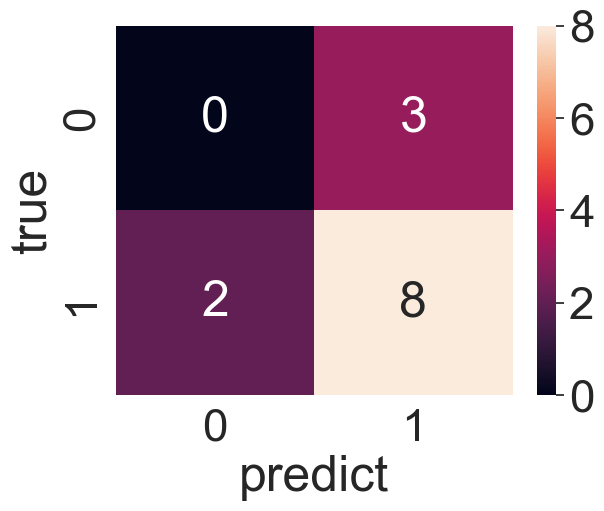
\includegraphics[width=0.8\textwidth]{LogisticRegression.png}
  \caption{LogisticRegression}
\end{figure}

\pagebreak
\subsection{correlation heatmap}


 A correlation heatmap is a graphical representation of the correlation between variables. The correlation coefficient is a measure of the linear relationship between two variables. It ranges from -1 to 1, where -1 indicates a perfect negative correlation, 0 indicates no correlation, and 1 indicates a perfect positive correlation.

The code first creates a figure with a width of 10 inches and a height of 7 inches. Then, it creates a heatmap of the correlation matrix of the DataFrame df. The annot=True argument causes the correlation coefficients to be displayed in the heatmap. Finally, the code sets the title of the figure to "Correlation between the columns" and displays the figure.

\begin{figure}[h!]
  \centering
  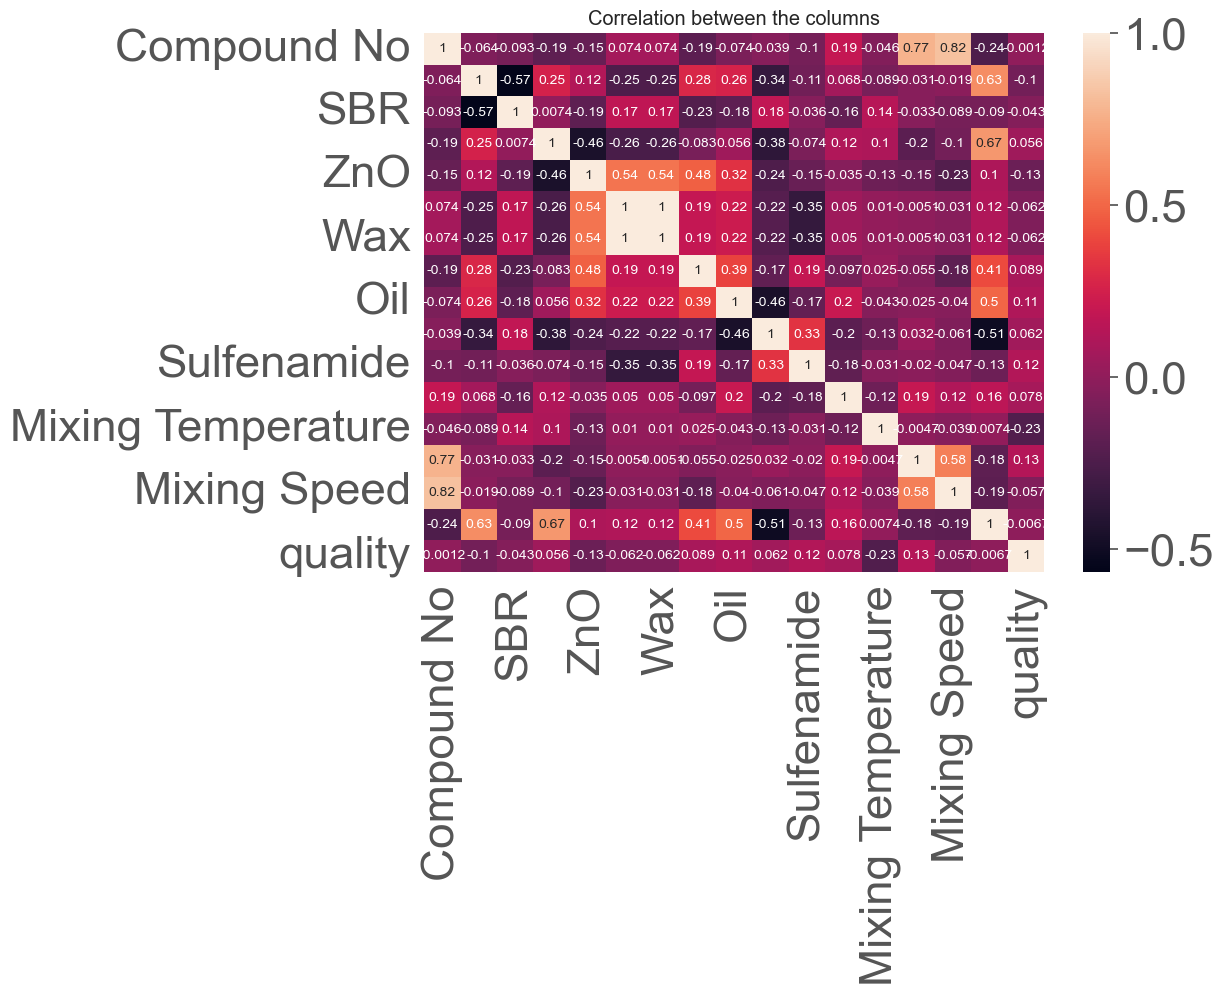
\includegraphics[width=0.8\textwidth]{Heatmap of Correlation Matrix.png}
  \caption{Heatmap of Correlation Matrix}
\end{figure}


\pagebreak
\subsection{Support Vector Machine Algorithm}

first checks for missing values in the DataFrame df and prints the number of missing values for each column. It then imports the StandardScaler class from the sklearn.preprocessing library, creates an instance of the class, and uses the $fit_transform()$ method to scale the features in the DataFrame df. The drop(labels=['quality'],axis=1) argument specifies that the quality column should not be scaled. The code then creates a new DataFrame $new_df$ with the scaled features. The $data=new_data$,columns=columns arguments specify the data and column names for the new DataFrame. Finally, the code uses the train$_test_split()$ function to split the data into a training set and a test set, and then uses the SVC class to train a support vector machine model on the training set. The code then uses the $accuracy_score()$ function to calculate the accuracy of the model on the test set. The output of the code is the accuracy of the model on the test set.

and i got accuracy of the model is: 0.9090909090909091

\subsection{KNN}

first imports the KNeighborsRegressor class from the sklearn.neighbors library, creates an instance of the class, and specifies the number of neighbors to use. It then splits the data into a training set and a test set, and then uses the fit() method to fit the model to the training set. The code then uses the predict() method to predict the target variable for the test set, and then uses the $r2_score()$ function to calculate the R2 score of the model. The output of the code is the R2 score of the model. the output is 0.03703703703703709.

\subsection{Naive Bayesian}

 imports the necessary libraries, then splits the data into input and target variables. Next, it splits the data into training and testing sets. Then, it initializes the Gaussian Naive Bayes model and fits it to the training data. Finally, it predicts the quality of the tyre compound using the test data and prints the accuracy of the model.and 
 Accuracy : 0.8461538461538461



 \section{Results and Discussions}

To evaluate the performance of each feature, I use differernt type of methods. such as Logistic regression, SVM, KNN , Naive Bayesian and ANN. i get the following results.

1. Random Forest accuracy : 76.92307692307693

2. logistic regression accuracy score:  61.53846153846154

3. Support Vector Machine Algorithm acuracy score : 90.90909090909091

4. Implementing Grid Search: 0.9090909090909091
5. KNN R2 score: 0.03703703703703709

6. Logistic regression accuracy: 0.9230769230769231
SVM accuracy: 0.9230769230769231









\section{References}
 \dots

\begin{enumerate}
\item https://www.gazityres.com/,
\item https://www.nokiantyres.com/innovation/facts-about-tyres/production-process/#:~:text=The%20main%20raw%20materials%20of,rubber%20from%20a%20rubber%20tree..





\item https://en.wikipedia.org/wiki/Tire manufacturing

\item
https://www.forest2market.com/blog/automotive-supply-chains-of-the-future-tyre-sector-circularity-0 

\item
https://www.ncbi.nlm.nih.gov/pmc/articles/PMC6465431/

\item
Landscape Applications of Machine
Learning: Comparing Random Forests
and Logistic Regression in Multi-Scale
Optimized Predictive Modeling of American
Marten Occurrence in Northern Idaho, USA


\item
https://en.wikipedia.org/wiki/Machine learning

\item
https://www.coursera.org/learn/machine-learning (Supervised Machine Learning: Regression and Classification)

\end{enumerate}








\end{document}